\let\lesson\undefined
\newcommand{\lesson}{\phantomlesson{Bài 9: Chuyển động ném}}
\chapter[Chuyển động ném xiên]{Chuyển động ném xiên}
\setcounter{section}{0}
\section{Lý thuyết}
\subsection{Chuyển động ném xiên}
Một chuyển động ném xiên cũng có thể  được phân tích thành hai thành phần: chuyển động thành phần theo phương thẳng đứng và chuyển động thành phần theo phương nằm ngang.
\begin{center}
	\begin{tikzpicture}[scale=1, transform shape]  %projectile motion
		\begin{axis}[
			width=10cm, %set bigger width
			height=5cm,
			xmin=0,xmax=11.5,
			ymin=0,ymax=4,
			xlabel=$x$,
			ylabel=$y$,
			axis x line = bottom,
			axis y line = left,
			axis line style={->},
			every axis y label/.style={at={(axis description cs:0,1.05)},anchor=south},
			every axis x label/.style={at={(axis description cs:1.02,0)},anchor=west},
			ticks = none,clip=false,
			]
			
			\tikzset{every mark/.append style={fill=red}}
			
			%variable definitions
			\def\g{-9.8} %gravity
			\def\v{10} %velocity
			\def\ang{51} %angle
			\def\s{0.2}
			\pgfmathsetmacro{\t}{0}
			%flight path
			\addplot[
			dashed,
			domain=0:10,
			samples=100,]
			{{\g*(x^2)/(2*\v^2*cos(\ang)^2)+x*tan(\ang)}};
			%			node[midway,above]{$V_y=0$};
			
			%vector at start
			\coordinate (A) at (axis cs: {\v*cos(\ang)*\t}, {\v*\t*sin(\ang)+0.5*\g*(\t^2)});
			\coordinate (B) at (axis cs: {\v*cos(\ang)*\t+\s*\v*cos(\ang)}, {\v*\t*sin(\ang)+0.5*\g*\t^2+\s*(\v*sin(\ang)+\g*\t)});
			\draw[thick,->](A)--(B)
			node[near end,above right=3mm and 0.5mm]{$\vec{v}_0$};
			\draw[densely dashed,thick,->](A)--(B|-A)
			node[near end,below]{$\vec{v}_{0x}$};
			\draw[densely dashed,thick,->](A)--(B-|A)
			node[near end,left]{$\vec{v}_{0y}$};
			
			\path plot[mark=*] coordinates {(A)};
			
			%dashed box around start vector
			\draw[dashed](B-|A)--(B);
			\draw[dashed](B|-A)--(B);
			
			%vector at end
			\pgfmathsetmacro{\a}{{-1*(2/\g)*\v*sin(\ang)}}
			\coordinate (E) at (axis cs:{\v*cos(\ang)*\a},{\v*\a*sin(\ang)+0.5*\g*(\a^2)}){};
			%			\coordinate (F) at (axis cs:{\v*cos(\ang)*\a+\s*\v*cos(\ang))}, {\v*\a*sin(\ang)+0.5*\g*\a^2+\s*(\v*sin(\ang)+\g*\a)});
			%			\draw[very thick,->](E)--(F)
			%			node[midway,sloped,above]{$V$};
			%			\draw[densely dashed,very thick,->](E)--(F |- E)
			%			node[midway,above]{$V_x$};
			%			\draw[densely dashed,very thick,->](E)--(F-| E)
			%			node[midway,left]{$V_y$};
			
			%			\path plot[mark=*] coordinates {(E)};
			
			%vector 1/2 up
			\pgfmathsetmacro{\b}{{(-1*(2/\g)*\v*sin(\ang))/4}}
			\coordinate (H) at (axis cs:{\v*cos(\ang)*\b},{\v*\b*sin(\ang)+0.5*\g*(\b^2)});
			\coordinate (I) at (axis cs: {\v*cos(\ang)*\b+\s*\v*cos(\ang)},{\v*\b*sin(\ang)+0.5*\g*\b^2+\s*(\v*sin(\ang)+\g*\b)});
			\draw[thick,->](H)--(I);
			%			node[midway,sloped,above]{$V$};
			\draw[densely dashed,thick,->](H)--(I-|H);
			%			node[midway,left]{$V_x$};
			\draw[densely dashed,thick,->](H)--(I|-H);
			%			node[midway,below]{$V_y$};
			
			\path plot[mark=*] coordinates {(H)};
			
			%vector halfway
			\pgfmathsetmacro{\c}{{(-1*(2/\g)*\v*sin(\ang))/2}}
			\coordinate (L) at (axis cs:{\v*cos(\ang)*\c},{\v*\c*sin(\ang)+0.5*\g*(\c^2)});
			\coordinate (M) at (axis cs:{\v*cos(\ang)*\c+\s*\v*cos(\ang))},{\v*\c*sin(\ang)+0.5*\g*\c^2+\s*(\v*sin(\ang)+\g*\c)});
			\draw[thick,->](L)--(M);
			%			node[near end,sloped,right=2mm]{$\vec{v}$};
			
			
			%T2 line; halfway up flight path
			\draw[loosely dashed,] (L) -- (axis cs:{\v*cos(\ang)*\c},0)
			node[midway,right] {$H$};
			
			
			\path plot[mark=*] coordinates {(L)};
			
			%vector 1/2 down
			\pgfmathsetmacro{\d}{{(-1*(2/\g)*\v*sin(\ang))*0.75}}
			\coordinate (P) at (axis cs:{\v*cos(\ang)*\d},{\v*\d*sin(\ang)+0.5*\g*(\d^2)});
			\coordinate (Q) at (axis cs:{(\v*cos(\ang)*\d+\s*\v*cos(\ang))},{\v*\d*sin(\ang)+0.5*\g*\d^2+\s*(\v*sin(\ang)+\g*\d)});
			\draw[thick,->](P)--(Q);
			%			node[midway,sloped,below]{$V$};
			\draw[densely dashed,thick,->](P)--(Q|-P);
			%			node[midway,above]{$V_x$};
			\draw[densely dashed,thick,->](P)--(Q-|P);
			%			node[midway,left]{$V_y$};
			
			\path plot[mark=*] coordinates {(P)};
			
			%start vector angle label
			\node[circle,minimum size=25pt] at (A) (circ) {};
			\node[right] at (circ.30) {$\theta$};
			\path[clip] (A) -- (B) -- (B|-A) -- cycle;
			\node[circle,draw,minimum size=25pt] at (A) (circ) {};
			
			%			\draw[<->,blue] (A)++(0,1cm) -- (E)++(0,1cm);
		\end{axis}
	\end{tikzpicture}	
	%	\begin{tikzpicture}[x=(330:1cm),y=(30:1cm),z=(90:1cm)]
		% green ground
		%		\fill [LightGreen] (-1,-1,0) -- (-.5,1,0) -- (11,2,0) -- (11,-2,0) -- cycle;
		%		\fill[Green] (9,0,0) circle [x radius=1.5, y radius=1];
		% black hole
		%		\fill[black] (10,0,0) circle [x radius=.1, y radius=.1];
		% red flag
		%		\draw[Brown, thick, line cap=round] (10,0,0) -- (10,0,1);
		%		\fill[Red] (10,0,1) -- (9.8,0,0.9) -- (10,0,0.8) -- cycle;
		% yellow sand hill
		%		\fill[Yellow, shift={(7,0,0)}] 
		%		plot [domain=0:340, samples=20, smooth cycle, variable=\t] 
		%		(\t:rnd/16+0.25 and rnd/8+0.75);
		
		% origin
		%		\node[below left] {$O$};
		% x-axis
		%		\draw (0, 0) -- (10, 0) 
		%		node[midway, yshift=-.8cm, rotate=330] {Distance, x (m)};
		%		\draw foreach \i in {2,4,6,8} 
		%		{ (\i, 0) node[below, rotate=330] {\i} -- ++(0, .15) };
		% y-axis
		%		\draw (0, 0, 0) -- (0, 0, 5) 
		%		node[pos=.8, xshift=-.8cm, rotate=90] {Height, y(m)};
		%		\draw foreach \i in {2,4} 
		%		{ (0, 0, \i) node[left] {\i} -- ++(.15, 0, 0) };
		
		%		\foreach \a[evaluate={\v=70; \T=\v*sin(\a)/9.807*2;}] in {60} {
			%			\draw[x=(330:0.5pt), z=(90:0.5pt), Black, dashed]
			%			plot [smooth, domain=0:\T, samples=50, variable=\t,
			%			mark=*, mark repeat=2, mark size=1.8pt, mark options={fill=white, solid}]
			%			(\v*\t*cos \a, 0, -9.807/2*\t^2+\v*\t*sin \a +0.1016) coordinate (end);
			%			\filldraw[fill=White] (end) circle [radius=1.8pt];
			%		}
		%	\end{tikzpicture}
\end{center}

%\begin{center}
%	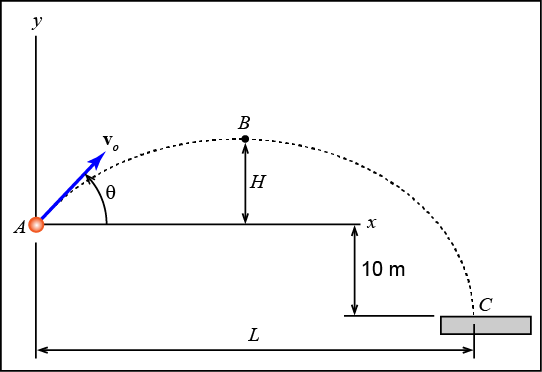
\includegraphics[scale=0.8]{../figs/G10-10-2}
%\end{center}

% Hung comment: hình vẽ G10-10-2 sai, không phù hợp với nội dung. Đã thay thế bằng hình vẽ với tikz pgfplot trên.		

\subsubsection{Tính chất của các chuyển động thành phần trên các trục}
\begin{itemize}
	\item Chuyển động thành phần theo trục O$x$ là chuyển động thẳng đều 
	\begin{align*}
		a_x&=0,\\
		v_x&=v_{0x}=v_0\cos\theta,\\
		x&=v_xt=v_0\left(\cos\theta\right) t.
	\end{align*}
	\item Chuyển động thành phần theo trục O$y$ là chuyển động rơi tự do có vận tốc đầu
	\begin{align}
		a_y&=-g,\\
		v_y&=v_{0y}-gt=v_0\sin\theta-gt,\\
		y&=v_{0y}t-\dfrac{1}{2}gt^{2}=v_0\left(\sin\theta\right) t-\dfrac{1}{2}gt^{2}.
	\end{align}
\end{itemize} 
\subsubsection{Độ cao cực đại}
Khi vật lên đến độ cao cực đại, thành phần vận tốc theo phương $y$ triệt tiêu. 
\begin{align*}
	H=y_{\max}=\dfrac{v_0^2\sin^2\theta}{2g}
\end{align*}

\subsubsection{Tầm xa}
\vspace{-0.5cm}
\begin{align*}
	L = x_{\max} = \dfrac{v_0^2 \sin 2\theta}{g}.
\end{align*}
\manatip{Với cùng một vị trí ném và cùng tốc độ đầu, tầm xa của vật ném xiên phụ thuộc vào góc ném. 

Vật đạt tầm xa cực đại nếu $\sin2\theta =1 \Leftrightarrow 2\theta=\SI{90}{\degree} \Leftrightarrow \theta=\SI{45}{\degree}$.}
\section{Mục tiêu bài học - Ví dụ minh hoạ}
\begin{dang}{Nhận biết các đặc điểm của chuyển động ném xiên}
	\viduii{2}
	{Trong chuyển động của vật được ném xiên từ mặt đất thì đại lượng nào sau đây không đổi?
		\begin{mcq}
			\item Gia tốc của vật.
			\item Độ cao của vật.
			\item Khoảng cách theo phương nằm ngang từ điểm vật được ném tới vật.
			\item Vận tốc của vật.
		\end{mcq}
	}
{\hide{
Trong chuyển động ném xiên từ mặt đất thì gia tốc của vật luôn bằng gia tốc rơi tự do và không đổi trong suốt quá trình vật chuyển động.\\
\textbf{Đáp án: A.}
}}
\viduii{3}
{Hai vật được ném đồng thời từ mặt đất lên với vận tốc ban đầu vẽ như Hình \ref{fig:13.1}. Nếu bỏ qua sức cản của không khí thì
	\begin{center}
		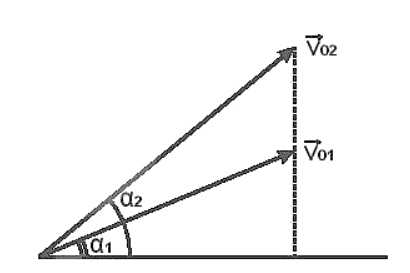
\includegraphics[width=0.3\linewidth]{../figs/VN10-2023-PH-TP013-1}
		\captionof{figure}{}
		\label{fig:13.1}
	\end{center}
	\begin{mcq}(2)
		\item vật 1 chạm đất trước.
		\item hai vật chạm đất cùng một lúc.
		\item hai vật có tầm bay cao như nhau.
		\item vật 1 có tầm bay cao hơn.
	\end{mcq}

}
{\hide{
Ta có toạ độ của vật ném xiên trên phương thẳng đứng
$$y=v_{0y}t-\dfrac{1}{2}gt^2$$
Khi vật chạm đất thì $y=0$
$$\Rightarrow t=\dfrac{2v_{0y}}{g}$$
Vì $v_{02y}>v_{01y}$ nên $t_2>t_1$. \\
Vậy vật 1 chạm đất trước.\\
\textbf{Đáp án: A.}

}}
\end{dang}
\begin{dang}{Xác định: độ cao cực đại, tầm xa, tốc độ chạm đất của vật trong chuyển động ném xiên}
	\viduii{3}
	{Một người nhảy xa với vận tốc ban đầu $\SI{7.5}{\meter/\second}$ theo phương xiên $\SI{30}{\degree}$ với phương nằm ngang. Biết vị trí dậm nhảy ngang với hố nhảy. Bỏ qua sức cản của không khí và lấy $g=\SI{9.8}{\meter/\second^2}$. Tính:
		\begin{enumerate}[label= \alph*)]
			\item Vận tốc ban đầu của người nhảy theo phương thẳng đứng và theo phương nằm ngang.
			\item Tầm cao $H$.
			\item Thời gian từ khi bắt đầu nhảy đến khi đạt độ cao cực đại.
			\item Thời gian từ lức bắt đầu nhảy lên đến khi rơi xuống hố nhảy.
			\item Tầm xa $L$.
		\end{enumerate}
	
}
{\hide{
Chọn hệ trục toạ độ $Oxy$ với $O$ là vị trí trên mặt đất mà người đó đặt chân vào để nhảy lên, trục $Oy$ thẳng đứng hướng lên, trục $Ox$ nằm ngang và cùng chiều tiến trên phương ngang của người.
\begin{center}
	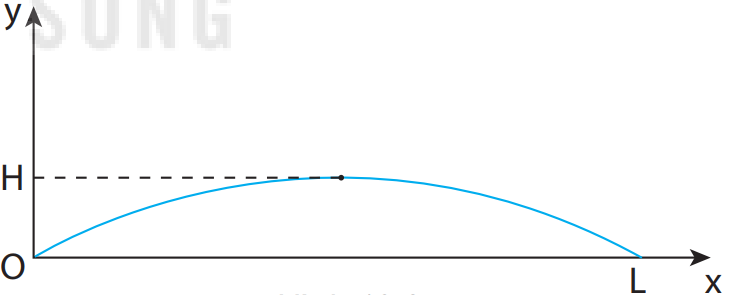
\includegraphics[width=0.4\linewidth]{../figs/VN10-2023-PH-TP013-2}
\end{center}
\begin{enumerate}[label=\alph*)]
	\item Vận tốc ban đầu
	\begin{align*}
		v_{0y}&=v_0\cdot\sin\SI{30}{\degree}=\SI{3.75}{\meter/\second}\\
		v_{0x}&=v_0\cos\SI{30}{\degree}=\SI{6.50}{\meter/\second}
	\end{align*}
\item Khi đạt tầm cao $H$ thì vận tốc của người nhảy theo phương thẳng đứng bằng $0$:
$$v^2_y-v^2_{0y}=2aH=-2gH$$
$$\Rightarrow H=\dfrac{v^2_{0y}}{2g}=\SI{0.717}{\meter}$$
\item Thời gian từ lúc bắt đầu nhảy đến khi đạt tầm cao cực đại
$$v_y=v_{0y}-gt\Rightarrow t =\dfrac{v_{0y}}{g}=\dfrac{\SI{3.75}{\meter/\second}}{\SI{9.8}{\meter/\second^2}}=\SI{0.383}{\second}$$
\item Thời gian từ lúc bắt đầu nhảy lên tới khi rơi xuống hố nhảy:
$$t'=2t=\SI{0.766}{\second}$$
\item Tầm xa:
$$L=d_\text{x max}=v_{0x}\cdot t'=\SI{4.98}{\meter}$$
\end{enumerate}
}}

\viduii{3}
{Người ta bắn một viên bi với vận tốc ban đầu $\SI{4}{\meter/\second}$ hướng lên cao theo phương xiên $\SI{45}{\degree}$ so với phương nằm ngang. Coi sức cản của không khí là không đáng kể.
	\begin{enumerate}[label=\arabic*.]
		\item Tính vận tốc của viên bi theo phương nằm ngang và phương thẳng đứng tại các thời điểm: bắt đầu bắn, sau $\SI{0.1}{\second}$ và sau $\SI{0.2}{\second}$.
		\item \begin{enumerate}[label=\alph*)]
			\item Viên bi đạt tầm cao $H$ vào lúc nào?
			\item Tính tầm cao $H$.
			\item Gia tốc của viên bi ở tầm cao $H$ có giá trị bằng bao nhiêu?
		\end{enumerate}
	\item \begin{enumerate}[label=\alph*)]
		\item Vận tốc của viên bi có độ lớn cực tiểu ở vị trí nào?
		\item Viên bi có vận tốc cực tiểu vào thời điểm nào?
	\end{enumerate}
\item \begin{enumerate}[label=\alph*)]
	\item Khi nào viên bi chạm sàn?
	\item Xác định vận tốc của viên bi khi chạm sàn.
	\item Xác định tầm xa $L$ của viên bi.
\end{enumerate}
	\end{enumerate}
}
{\hide{
Chọn hệ trục toạ độ $Oxy$ như hình vẽ, gốc toạ độ tại vị trí ban đầu của viên bi, gốc thời gian lúc bắn viên bi.
\begin{enumerate}[label=\arabic*.]
	\item \begin{itemize}
		\item Thời điểm ban đầu:
		\begin{itemize}
			\item Vận tốc của viên bi theo phương ngang
			$$v_{0x}=v_0\cos\SI{45}{\degree}=\xsi{2\sqrt{2}}{\meter/\second}$$
			Vận tốc của viên bi theo phương thẳng đứng:
			$$v_{0y}=v_0\sin\SI{45}{\degree}=\xsi{2\sqrt{2}}{\meter/\second}$$
		\end{itemize}
	\item Sau $\SI{0.1}{\second}$
	\begin{itemize}
		\item Vận tốc của viên bi theo phương ngang:
		$$v_x=v_{0x}=\xsi{2\sqrt{2}}{\meter/\second}$$
		\item Vận tốc của viên bi theo phương thẳng đứng:
		$$v_y=v_{0y}-gt=\left(\xsi{2\sqrt{2}}{\meter/\second}\right)-\left(\SI{9.8}{\meter/\second^2}\right)\cdot\left(\SI{0.1}{\second}\right)=\SI{1.85}{\meter/\second}$$
	\end{itemize}
	\item Sau $\SI{0.2}{\second}$
	\begin{itemize}
		\item Vận tốc của viên bi theo phương ngang:
		$$v_x=v_{0x}=\xsi{2\sqrt{2}}{\meter/\second}$$
		\item Vận tốc của viên bi theo phương thẳng đứng:
		$$v_y=v_{0y}-gt=\left(\xsi{2\sqrt{2}}{\meter/\second}\right)-\left(\SI{9.8}{\meter/\second^2}\right)\cdot\left(\SI{0.2}{\second}\right)=\SI{0.87}{\meter/\second}$$
	\end{itemize}
	\end{itemize}
\item \begin{enumerate}[label=\alph*)]
	\item Khi đạt tới tầm cao $H$ thì 
	$$v_y=v_{0y}-gt=0\Rightarrow t=\dfrac{v_{0y}}{g}=\dfrac{\xsi{2\sqrt{2}}{\meter/\second}}{\SI{9.8}{\meter/\second^2}}=\SI{0.289}{\second}$$
	\item Tầm cao 
	$$H=\dfrac{v^2_{0y}}{2g}=\dfrac{\left(\xsi{2\sqrt{2}}{\meter/\second}\right)^2}{2\cdot\left(\SI{9.8}{\meter/\second^2}\right)}=\SI{0.408}{\meter}$$
	\item Gia tốc của viên bi ở tầm cao $H$:
	$$a=g=\SI{9.8}{\meter/\second^2}$$
	Khi đạt độ cao cực đại, viên bi bắt đầu rơi xuống do tác dụng của trọng lực.
\end{enumerate}
\item \begin{enumerate}[label=\alph*)]
	\item Thời gian kể từ lúc bắn viên bi lên đến khi viên bi chạm sàn bằng 2 lần thời gian kể từ lúc bắn viên bi lên đến khi nó đạt độ cao cực đại
	$$t'=2t=2\cdot\left(\SI{0.289}{\second}\right)=\SI{0.578}{\second}$$
	\item Khi chạm sàn
	
	Thành phần vận tốc của viên bi trên phương ngang có độ lớn
	$$v_x=v_{0x}=\xsi{2\sqrt{2}}{\meter
	/\second}$$
	Thành phần vận tốc của viên bi trên phương thẳng đứng có độ lớn
	$$v_y=\sqrt{2gH}\approx\SI{2.83}{\meter/\second}$$
	Tốc độ của viên bi khi chạm sàn
	$$v=\sqrt{v^2_x+v^2_y}=\sqrt{\left(\xsi{2\sqrt{2}}{\meter/\second}\right)^2+\left(\SI{2.83}{\meter/\second}\right)^2}\approx\SI{4}{\meter/\second}$$
	\item Tầm xa 
	$$L=d_{x \text{max}}=v_{0x}\cdot t'=\left(\xsi{2\sqrt{2}}{\meter/\second}\right)\cdot\left(\SI{0.578}{\second}\right)=\SI{1.635}{\meter}$$
\end{enumerate}
\end{enumerate}
}}
\end{dang}
